\documentclass[t]{beamer}
\usetheme{Copenhagen}
\setbeamertemplate{headline}{} % remove toc from headers
\beamertemplatenavigationsymbolsempty

\usepackage{amsmath, array, tikz, bm, pgfplots, tcolorbox, graphicx}
\pgfplotsset{compat = 1.16}
\usepgfplotslibrary{statistics}


\title{Measures of Position}
\author{}
\date{}

\AtBeginSection[]
{
  \begin{frame}
    \frametitle{Objectives}
    \tableofcontents[currentsection]
  \end{frame}
}

\begin{document}

\begin{frame} 
\maketitle
\end{frame}

\section{Use z-scores to compare data values}

\begin{frame}{z-scores}
\begin{tcolorbox}[colframe=green!20!black, colback = green!30!white,title=\textbf{z-score}]
A \textbf{z-score} (a.k.a. \textbf{standard score}) measures how many standard deviations a data value, $x$, is from the mean of the data set.
\end{tcolorbox}
\vspace{8pt}	\pause
\begin{itemize}
	\item A positive z-score indicates an above average value.	\newline\\	\pause
	\item A negative z-score indicates a below average value.	\newline\\	\pause
	\item A z-score of 0 indicates an exact average value.
\end{itemize}
\end{frame}

\begin{frame}{Visual Interpretation of z-Scores}
\begin{center}
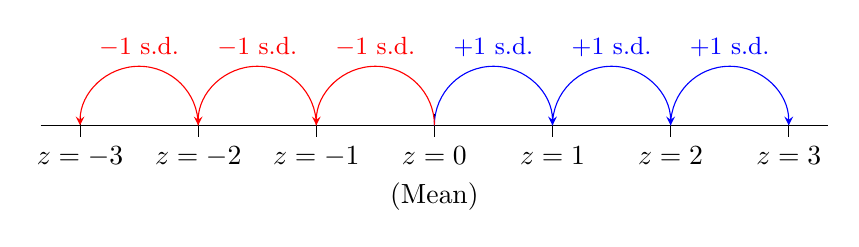
\begin{tikzpicture}
\draw (-5,0) -- (5,0);
\foreach \x in {-4.5,-3,...,4.5}
\draw (\x, 0.15) -- (\x, -0.15);
\node at (0,-0.15) [below] {$z=0$};
\node at (0,-0.6) [below] {(Mean)};
\node at (1.5,-0.15) [below] {$z=1$};
\draw [->, >=stealth,blue] (0,0) arc (180:0:0.75) node [above, midway] {\small$+1\text{ s.d.}$};
\node at (3,-0.15) [below] {$z=2$};
\draw [->, >=stealth,blue] (1.5,0) arc (180:0:0.75) node [above, midway] {\small$+1\text{ s.d.}$};
\node at (4.5,-0.15) [below] {$z=3$};
\draw [->, >=stealth,blue] (3,0) arc (180:0:0.75) node [above, midway] {\small$+1\text{ s.d.}$};
\node at (-1.5,-0.15) [below] {$z=-1$};
\draw [->, >=stealth, red] (0,0) arc (0:180:0.75) node [above, midway] {\small$-1\text{ s.d.}$};
\node at (-3,-0.15) [below] {$z=-2$};
\draw [->, >=stealth, red] (-1.5,0) arc (0:180:0.75) node [above, midway] {\small$-1\text{ s.d.}$};
\node at (-4.5,-0.15) [below] {$z=-3$};
\draw [->, >=stealth, red] (-3,0) arc (0:180:0.75) node [above, midway] {\small$-1\text{ s.d.}$};
\end{tikzpicture}
\end{center}
\end{frame}

\begin{frame}{z-Score Formula}
\[z = \frac{x-\mu}{\sigma}\]	\pause

z-scores can compare two different data sets that use different scales of measurement.	\newline\\	\pause

``Usual" data values have z-scores between $-2$ and 2.
\end{frame}

\begin{frame}{Example 1}
The mean SAT score is 1059 with a standard deviation of 210; meanwhile the mean ACT score is 21 with a standard deviation of 5.4. A student takes both tests and receives a 1350 on the SAT and a 29 on the ACT. On which test did the student score better? \\
\begin{align*}
\onslide<2->{z_{\text{SAT}} &= \frac{1350-1059}{210}}	&	\onslide<4->{z_{\text{ACT}} &= \frac{29-21}{5.4}}	\\[10pt]
\onslide<3->{z_{\text{SAT}} &= 1.39}					&	\onslide<5->{z_{\text{ACT}} &= 1.48}	\\
\end{align*}
\onslide<6->{The student did relatively better on the ACT.}
\end{frame}


\section{Determine and interpret percentiles}

\begin{frame}{Percentiles}
\begin{tcolorbox}[colframe=green!20!black, colback = green!30!white,title=\textbf{Percentile}]
A \textbf{percentile} is a measure of location that divide a set of data into 100 groups with about 1\% of the values in each group.
\end{tcolorbox}
\vspace{11pt} \pause

\begin{tcolorbox}[colframe=green!20!black, colback = green!30!white,title=\textbf{Percentile Score}]
A \textbf{percentile score} is the percent of data values less than a given value. (\emph{Note}: this is \underline{not} the same as percentage).
\end{tcolorbox}
\vspace{11pt} \pause

\emph{Note:} There is no universally agreed method to calculate percentiles.
\end{frame}

\begin{frame}{Example 2}
Explain the difference between getting 90\% on a test and scoring in the 90th percentile on that test.	\newline\\	\pause

Getting 90\% means you earned 90\% of the total points available for that test.	\newline\\	\pause

Scoring in the 90th percentile means that you did better than 90\% of all other test takers.
\end{frame}

\section{Determine the five-number summary}

\begin{frame}{Quartiles}
\begin{tcolorbox}[colframe=green!20!black, colback = green!30!white,title=\textbf{Quartiles}]
\textbf{Quartiles} are values that divide a data set into 4 groups, with each group holding 25\% of the data.
\end{tcolorbox}
\vspace{8pt}	\pause
\begin{center}
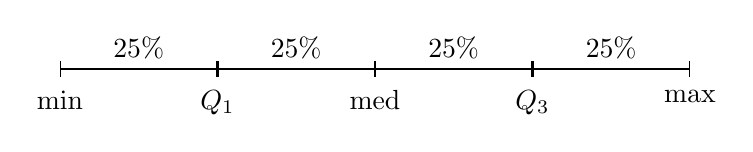
\begin{tikzpicture}
\coordinate (A) at (0,0);
\coordinate (B) at (2,0);
\coordinate (C) at (4,0);
\coordinate (D) at (6,0);
\coordinate (E) at (8,0);
\draw[|-|] (A) node [below, yshift=-0.15cm] {min} -- (B) node [midway, above] {25\%};
\draw[|-|] (B) node [below, yshift=-0.15cm] {$Q_1$} -- (C) node [midway, above] {25\%};
\draw[|-|] (C) node [below, yshift=-0.15cm] {med} -- (D) node [midway, above] {25\%};
\draw[|-|] (D) node [below, yshift=-0.15cm] {$Q_3$} -- (E) node [midway, above] {25\%};
\node at (E) [below, yshift=-0.15cm] {max};
\end{tikzpicture}
\end{center}
\vspace{8pt} \pause
$Q_1$ is called the first (a.k.a. \textit{lower}) quartile and $Q_3$ is called the third (a.k.a. \textit{upper}) quartile.
\end{frame}

\begin{frame}{Five-Number Summary}
\begin{tcolorbox}[colframe=green!20!black, colback = green!30!white,title=\textbf{Five-Number Summary}]
The \textbf{five-number summary} are the following values: 
\begin{center}
Minimum, $Q_1$, Median, $Q_3$, Maximum
\end{center}
\end{tcolorbox}
\end{frame}

\begin{frame}{Example 3}
Find the five-number summary of the following dataset:	
\begin{center}
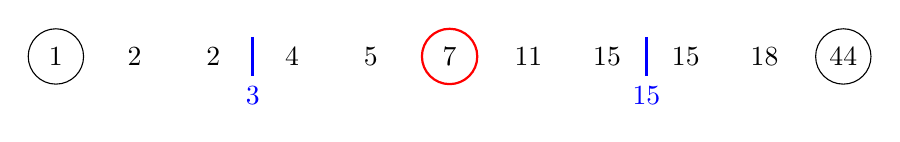
\begin{tikzpicture}
\node at (0,0) {1};
\node at (1,0) {2};
\node at (2,0) {2};
\node at (3,0) {4};
\node at (4,0) {5};
\node at (5,0) {7};
\node at (6,0) {11};
\node at (7,0) {15};
\node at (8,0) {15};
\node at (9,0) {18};
\node at (10,0) {44};
\onslide<2->{\draw (0,0) circle [radius = 10pt];}
\onslide<3->{\draw (10,0) circle [radius = 10pt];}
\onslide<4->{\draw[color=red, thick] (5,0) circle [radius=10pt];}
\onslide<5->{\draw[very thick, color=blue] (2.5,0.25) -- (2.5,-0.25) node [below] {3};}
\onslide<6->{\draw[very thick, color=blue] (7.5,0.25) -- (7.5,-0.25) node [below] {15};}
\end{tikzpicture}
\end{center}
\vspace{8pt} \pause
\onslide<2->{Minimum: 1}	\newline\\	
\onslide<5->{First quartile: 3} \newline\\ 
\onslide<4->{Median: 7}	\newline\\	
\onslide<6->{Third quartile: 15} \newline\\	
\onslide<3->{Maximum: 44}
\end{frame}

\begin{frame}{Outliers}
\begin{tcolorbox}[colframe=green!20!black, colback = green!30!white,title=\textbf{Outliers}]
An outlier is an extreme data value in a dataset.
\end{tcolorbox}
\vspace{8pt} \pause
We can use the five-number summary to detect outliers.	\newline\\	\pause
\begin{tcolorbox}[colframe=green!20!black, colback = green!30!white,title=\textbf{Interquartile Range}]
The \textbf{interquartile range} can be found by subtracting $Q_1$ from $Q_3$:
\[ \text{IQR} = Q_3 - Q_1 \]
\end{tcolorbox}
\end{frame}

\begin{frame}{Lower and Upper Fences}
The {\color{blue}\textbf{lower fence}} is
\[Q_1 - 1.5(\mathrm{IQR}) \]
and the {\color{blue}\textbf{upper fence} is}
\[Q_3 + 1.5(\mathrm{IQR}) \]
\pause

A data value is an {\color{red}\textbf{outlier}} if it is less than the lower fence or more than the upper fence.
\end{frame}

\begin{frame}{Example 4}
Calculate the lower and upper fences of the previous example's dataset and use it to find any outliers.	
\begin{center}
1, 2, 2, 4, 5, 7, 11, 15, 15, 18, 44
\end{center}
\begin{align*}
	\onslide<2->{\text{Lower fence} &= Q_1 - 1.5(IQR)} \\
	\onslide<3->{&= 3 - 1.5(15-3)} \\
	\onslide<4->{&= -15}
\end{align*}
\begin{align*}
	\onslide<2->{\text{Upper fence} &= Q_3 + 1.5(IQR)} \\
	\onslide<3->{&= 15 + 1.5(12)} \\
	\onslide<4->{&= 33}
\end{align*}
\end{frame}

\begin{frame}{Example 4}
\begin{center}
\begin{tikzpicture}
\draw[|-|] (0,0) node [below, yshift=-0.15cm] {$-15$} -- (4,0) node [below, yshift=-0.15cm] {$33$};
\draw[fill] (6,0) circle [radius = 2pt] node [below, yshift=-0.15cm] {44};
\end{tikzpicture}
\end{center}	\vspace{8pt} \pause
44 is an outlier of the dataset
\end{frame}

\section{Create a boxpolot of a dataset}

\begin{frame}{Boxplots}
\begin{tcolorbox}[colframe=green!20!black, colback = green!30!white,title=\textbf{Boxplot}]
A \textbf{boxplot} is a visual display of the five-number summary. 
\end{tcolorbox}
\vspace{8pt}	\pause
\begin{center}
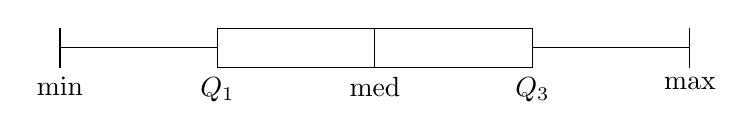
\begin{tikzpicture}
\draw (0,0.25) -- (0,-0.25) node [below] {min};
\draw (2,0.25) -- (2,-0.25) node [below] {$Q_1$};
\draw (4,0.25) -- (4,-0.25) node [below] {med};
\draw (6,0.25) -- (6,-0.25) node [below] {$Q_3$};
\draw (8,0.25) -- (8,-0.25) node [below] {max};
\draw (2,-0.25) rectangle (6,0.25);
\draw (0,0) -- (2,0);
\draw (6,0) -- (8,0);
\end{tikzpicture}
\end{center}
\end{frame}

\begin{frame}{Example 5}
Create a boxplot of the dataset
\begin{center}
1, 2, 2, 4, 5, 7, 11, 15, 15, 18, 44
\newline\\ \pause
Min = 1 \quad $Q_1 = 3$ \quad Med = 7 \quad $Q_3 = 15$ \quad Max = 44
\newline\\	\pause
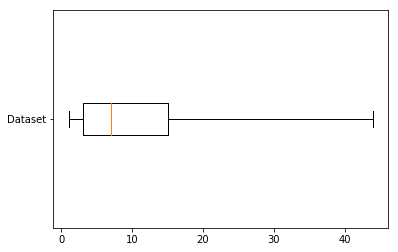
\includegraphics[scale=0.5]{../Images/boxplot.png}
\end{center}
\end{frame}

\begin{frame}{Modified Boxplot}
With a modified boxplot, outliers are shown with symbols such as stars or points. \newline\\	\pause

Whiskers are drawn out to the points that are {\color{blue}\textbf{not}} considered outliers.	
\end{frame}

\begin{frame}{Modified Boxplot}
\begin{center}
1, 2, 2, 4, 5, 7, 11, 15, 15, 18, 44	\newline\\
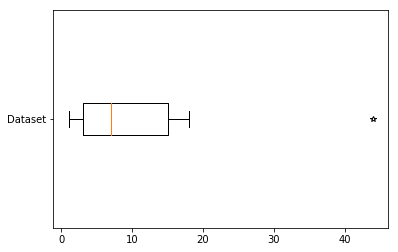
\includegraphics[scale=0.5]{../Images/modified_boxplot.png}
\end{center}
\end{frame}



\end{document}